\chapter{Methods} \label{ch:methods}

Analyses in large experiments and particle colliders are often several steps removed from the direct measuring tools of the experiment. The raw data are measured and recorded by the detector, then the signals are processed and analyzed by a combination of hardware and software to reconstruct the data that represents a physical object, such as a particle, or a jet. Physical observables are then calculated from the reconstructed data and used to draw conclusions. The following sections describe the reconstruction process and the observables used in this analysis.

\section{Data}

The data used in this analysis were measured in 2017 and 2018 during Run 2 of the LHC. The data were measured from proton-proton collisions at a center-of-mass energy of $\sqrt{s} = 2.01$ TeV and lead-lead collisions at $\sqrt{s_{NN}} = 5.02$ TeV. The data were collected by the ALICE detector using a minimum bias trigger for the proton-proton events, and a centrality trigger for the lead-lead events, in addition to the minimum bias trigger. This analysis studies 0-10\% centrality collisions, referred to as central events throughout, and 30-50\% centrality collisions, referred to as semicentral collisions throughout. We used XXM events in the proton-proton sample, XXM events in the central lead-lead sample, and XXM events in the semicentral lead-lead sample.

\section{Reconstruction}

The raw detector data go through several steps to reconstruct the data that represent physical objects. The raw signals are first aggregated into local clusters within each detector, and referred to as hits. The hits are then used as input to reconstruct tracks, the trails of hits left behind by a charged particle, and vertices, the collision locations. From the reconstructed tracks, we can reconstruct jets and calculate jet observables. Some of these steps are carried out in hardware circuits and others are done long after the data are measured, in software. There are many nuances in the reconstruction process beyond the scope of this thesis. The interested reader can see the official ALICE reconstruction documentation~\cite{ALICEreco}.

\subsection*{Vertex Reconstruction}

The primary vertices, the locations of the collision for each event, are randomly distributed about the center of the detector along the x, y, and z directions. Each collision system will have a different beam profile resulting in a different distribution of primary vertices. The innermost layers of the ITS are used to measure the distributions of particle positions near the primary vertex in both the transverse and longitudinal directions. Once tracks have been reconstructed, we can provide a better estimate of the primary vertex location by projecting the tracks back to point of convergence. This improves the primary vertex resolution by a factor of two~\cite{trackVertexReconstruction}.

\subsection*{Track Reconstruction}

Tracking refers to the process of taking all of the hits, clusters of signals left by particles, measured in various detectors during a single event and reconstructing the path that each particle took through the detector volume. This can be done globally, considering all hits and simultaneously reconstructing all particle trajectories. Alternatively, tracking can be done locally, building particle trajectories one step at a time. The ALICE detector uses a local tracking method that iteratively applies a Kalman Filter to reconstruct particle trajectories. A detailed discussion of Kalman Filtering can be found in~\cite{Kalman}.
The first step in track reconstruction is cluster finding, where the raw detector signals are grouped together into clusters, which are assumed to represent a particle hit in the active detector volume. Some corrections are applied the to the cluster position arising from the details of the detectors, like TPC space-charge corrections, and overlapping clusters. The next step is track finding, where the clusters are grouped together into track candidates. The algorithm starts by finding ”seed tracks” which can be followed and combined with clusters to produce the final track. These seed tracks can be found in different ways. One can apply a vertex constraint and generate seed tracks using clusters close to the primary vertex that project back to it, and then add clusters in the outer TPC that lie in a small window projected from the primary vertex along the other cluster locations. Alternatively, one can start in the middle of the TPC and find clusters that are nearby to each other until a stopping condition is met. These methods are complementary as some tracks require a primary vertex constraint, while other tracks will suffer from the use of such a constraint. Once the seed tracks are found, they are followed in multiple passes to the innermost and outermost layers of the TPC. Along the way, clusters are considered if they are within 4$\sigma$ of the current track, and the nearest cluster is accepted as the most probable cluster for that track. Tracks are then further extended into the ITS using the Kalman Filtering approach that is slightly modified to account for the increased occupancy in the ITS, as well as the dead zone between the ITS and the TPC. The tracks are finally propagated out to the outermost detectors, including the TRD and TOF. In addition to position information, momentum information and several other observables related to particle identification are also calculated and assigned to the track.

\subsection*{Jet Reconstruction}
After tracks have been reconstructed they can be clustered into jets using the anti-$k_T$ algorithm. The anti-$k_T$ algorithm is implemented in the FastJet v3.4 software package~\cite{FastJet}. We measure full jets in this analsysis for the closest comparison with theory and simulations. In order to minimize the impact of combinatorial jets, we use liberal cuts to reduce combinatorial jet population. First, we only cluster tracks with $p_T$ $\geq$ 3GeV/c when clustering our jets. Additionally, we require that every jet contain at least one track with $p_T$ $\geq$ 5 GeV/c. These cuts dramatically reduce the impact of combinatorial jets on our results. Once jets have been clustered, we use the ALICE area-based background subtraction method. In this method, we assume that the background contribution to a jet is proportional to the area of that jet. The background momentum density per unit area ($\rho$) is measured using the $k_T$ jet-finding algorithm. $\rho$ is estimated as the median of the $p_T$ per unit area of jets after throwing out the two highest momentum jets in the event.

\section{Jet Hadron Correlation Functions}
 The process of jet reconstruction and the cuts applied to the jets result in a population of jets that are less modified by the medium than the average jet. In order to remove this bias, we measure the jet-hadron correlation function. Jet-hadron correlation functions measure the density of hadrons per jet in azimuth, $\phi$, and pseudorapidity, $\eta$. In order to average over all jets, we actually measure the hadron density in ($\Deta$, $\Dphi$), where $\Deta$ = $\eta$ - $\eta_{jet}$ and $\Dphi$ = $\phi$ - $\phi_{jet}$. This results in a map of our detector showing us where the hadrons are relative to the jets. The jet-hadron correlation function is defined as 

\begin{equation}
    \rho(\Delta \eta, \Delta \phi) = \frac{1}{N_{jets}} \frac{d^2N_{assoc.}}{d\Delta \eta d\Delta \phi}
\end{equation}

\noindent where $N_{jets}$ is the number of jets, and $N_{assoc.}$ is the number of hadrons associated with a jet. The jet-hadron correlation function is usually measured in bins of jet momentum and associated hadron momentum. In this analysis, we have two jet momentum bins and seven associated hadron momentum bins, summarized in Table~\ref{tab:jetHadronBins}. 

\begin{table}
    \centering
    \begin{tabular}{|c||c|}
        \hline
        Jet Momentum Bins & Associated Hadron Momentum Bins \\
        \hline
        20-40 GeV/c & 1-1.5 GeV/c \\
        40-60 GeV/c & 1.5-2 GeV/c \\
        & 2-3 GeV/c \\
        & 3-4 GeV/c \\
        & 4-5 GeV/c \\
        & 5-6 GeV/c \\
        & 6-10 GeV/c \\
        \hline
    \end{tabular}
    \caption{Jet momentum and associated hadron momentum bins used in this analysis.}\label{tab:jetHadronBins}
\end{table}

There are two corrections to the jet-hadron correlation function which correct for single-track and track pair reconstruction inefficiency. The single track reconstruction efficiency measures the probability that a track is reconstructed in the detector at a particular $p_T$ and $\eta$. The pair acceptance efficiency measures the probability that a jet-hadron pair is reconstructed in the detector at a particular jets and hadron $p_T$, $\Deta$, and $\Dphi$.  The jet-hadron correlation function is corrected for the single track reconstruction efficiency and pair acceptance efficiency by

\begin{equation}
    \rho_{corr.}(\Deta, \Dphi) = \frac{\rho_{meas.}(\Delta \eta, \Delta \phi)}{\epsilon_{single}(\eta_{assoc.}, p_{T,assoc.}) \epsilon_{pair}(\Deta, \Dphi, p_{T,assoc.}, p_{T,jet})}
\end{equation}

\noindent where $\epsilon_{single}$ is the single track reconstruction efficiency, and $\epsilon_{pair}$ is the pair acceptance efficiency.

In addition to the efficiency corrections described above, the jet-hadron correlation function is also corrected for the background: hadrons arising from non-jet sources. In the region 0.8$geq$ |$\Deta$| $\leq$1.2 and $-\pi$/2$\leq$ $\Dphi$ $\leq$ $\pi$/2, the jet-hadron correlation function is dominated by the background. The background contribution across the entire jet-hadron correlation function is estimated from this region and subtracted from the jet-hadron correlation function. 

\subsection*{Charged Track Reconstruction Efficiency}

Due to the finite global acceptance and finite tracking efficiency of the ALICE detector, the raw correlations must be corrected for the single track reconstruction efficiency. The single track reconstruction efficiency is defined as the probability that a charged particle produced in the collision will be reconstructed as a track in the detector. The single track reconstruction efficiency for this analysis has been measured for the Pb Pb collisions and is the same as in~\cite{CharlesThesis}, shown in Figure~\ref{fig:STRE}. The single track reconstruction efficiency is measured as a function of $p_T$ and $\eta$ for each collision system. The single track reconstruction efficiency is measured using Monte-Carlo simulations of the ALICE detector and the HIJING event generator~\cite{HIJING}. Particles are generated and propagated through the detector simulationand the probability of reconstructing those particles is measured.  

\begin{figure}
    \centering
    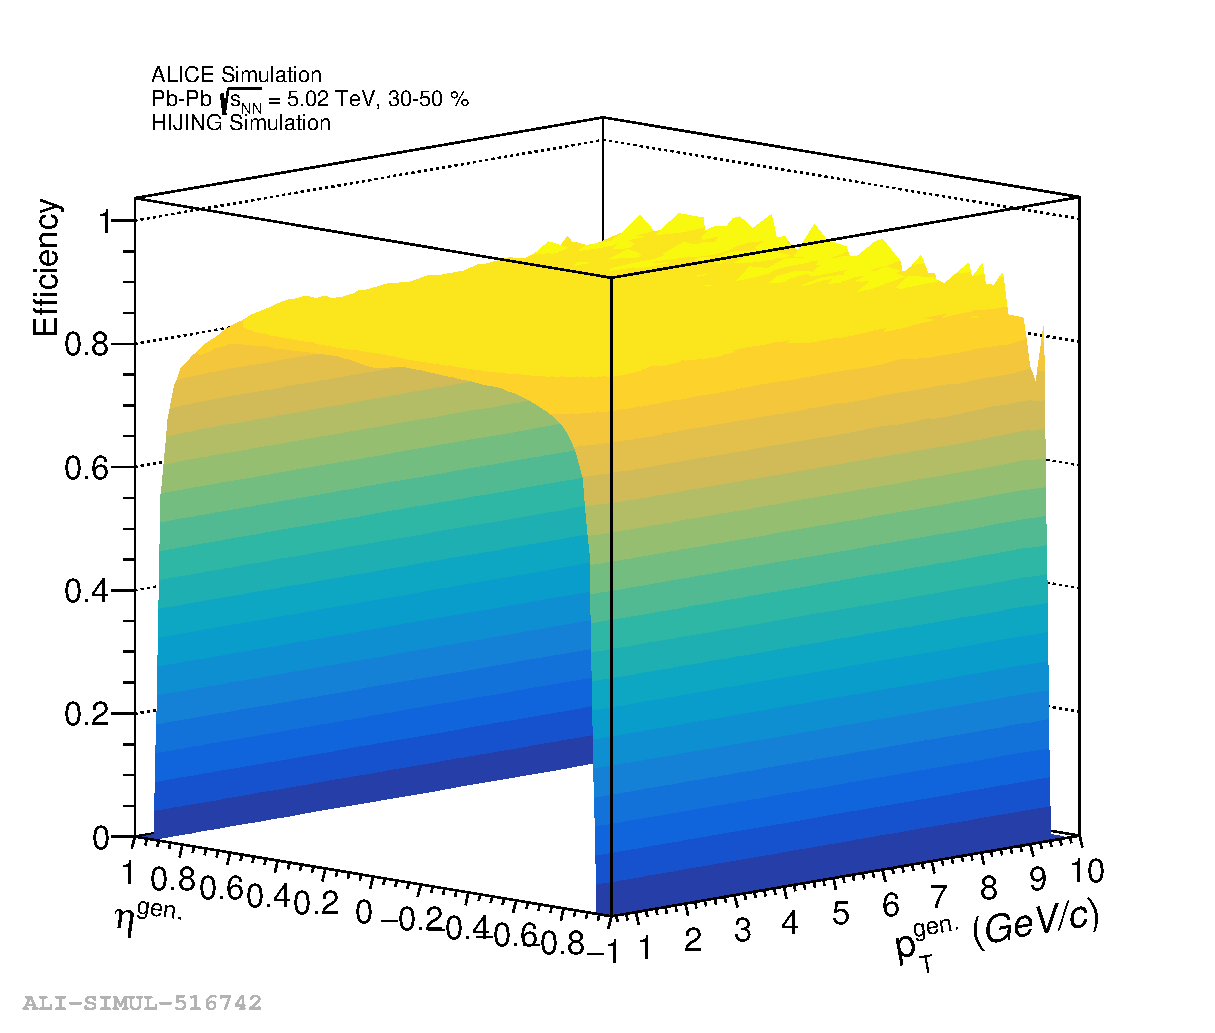
\includegraphics[width=0.8\textwidth]{figures/eps/Prelim_Approval_STRE_2.eps}
    \caption{Single track reconstruction efficiency as a function of $p_T$ and $\eta$ for Pb Pb collisions.}\label{fig:STRE}
\end{figure}